\documentclass[border=4pt,12pt]{standalone}
% House style for redrawn exam diagrams (diagram-v4: 0.4pt lines, filled -latex arrows, fine dashes; stipple and hatching drawn as real dots/lines (no PDF/SVG patterns, so they render in every browser and at any scale); transparent background). Every figure \input's this.
\usepackage{amsmath,amssymb}
\usepackage{txfonts}
\usepackage{pdfrender,xcolor}
% \halo{text}: label on shading. The shading stops just around each letter's outline (a thin knock-out that follows the
% glyphs, like the papers' typesetting), never a box. Owner: "I don't want a box around the text".
\newcommand{\halo}[1]{\leavevmode\rlap{\pdfrender{TextRenderingMode=2,LineWidth=2.2pt,LineJoinStyle=1,StrokeColor=white,FillColor=white}#1}#1}
\usepackage{tikz,pgfplots}
\pgfplotsset{compat=1.18}
\usetikzlibrary{arrows.meta,calc,angles,quotes,patterns,patterns.meta,intersections,positioning,decorations.markings,shapes.geometric}
% Stipple and hatching are drawn as actual dots / lines clipped to the region (path picture), NOT as pattern fills:
% SVG <pattern> fills vanish or blur when browsers scale the image, so the owner could not see the shading.
% Each dot is a 0.72pt square (keeps SVGs small; reads as a dot at print size). Dots sit on one global staggered grid, so neighbouring regions line up.
\makeatletter
\newdimen\ex@x \newdimen\ex@y \newdimen\ex@xa \newdimen\ex@ya \newdimen\ex@xb \newdimen\ex@yb \newcount\ex@row
\def\exam@stipplecolor{black!75}\def\exam@dotr{0.42pt}\def\exam@dotgap{2.5}
\def\ex@rowdots{\ifdim\ex@x<\ex@xb \pgfpathrectangle{\pgfqpoint{\dimexpr\ex@x-0.36pt\relax}{\dimexpr\ex@y-0.36pt\relax}}{\pgfqpoint{0.72pt}{0.72pt}}\advance\ex@x by \exam@dotgap pt\relax\expandafter\ex@rowdots\fi}
\def\exam@stipple{%
  \pgftransformreset% dots are sized in real points even inside scaled pictures
  \pgfpointanchor{path picture bounding box}{south west}\ex@xa=\pgf@x \ex@ya=\pgf@y
  \pgfpointanchor{path picture bounding box}{north east}\ex@xb=\pgf@x \ex@yb=\pgf@y
  \pgfsetfillcolor{\exam@stipplecolor}\pgfmathsetmacro\ex@h{\exam@dotgap/2}%
  \pgfmathtruncatemacro\ex@r{floor(\ex@ya/\ex@h)-1}\ex@row=\ex@r\relax
  \ex@y=\ex@r\dimexpr\ex@h pt\relax
  \loop\ifdim\ex@y<\ex@yb
    \pgfmathtruncatemacro\ex@c{floor(\ex@xa/\exam@dotgap)-1}\ex@x=\ex@c\dimexpr\exam@dotgap pt\relax
    \ifodd\ex@row \advance\ex@x by \ex@h pt\fi
    \ex@rowdots
    \advance\ex@y by \ex@h pt \advance\ex@row by 1
    \ifnum\numexpr\ex@row-(\ex@row/4)*4\relax=0 \pgfusepath{fill}\fi% flush every 4 rows: bounded TeX memory, few clip copies in the SVG
  \repeat\pgfusepath{fill}}
\newdimen\ex@d
\def\exam@hatch#1{% #1 = 1 for /, -1 for \ ; lines 45 degrees, 3pt apart
  \pgftransformreset
  \pgfpointanchor{path picture bounding box}{south west}\ex@xa=\pgf@x \ex@ya=\pgf@y
  \pgfpointanchor{path picture bounding box}{north east}\ex@xb=\pgf@x \ex@yb=\pgf@y
  \ex@d=\dimexpr\ex@yb-\ex@ya\relax \ex@x=\dimexpr\ex@xa-\ex@d\relax
  \loop\ifdim\ex@x<\ex@xb
    \ifnum#1>0 \pgfpathmoveto{\pgfqpoint{\ex@x}{\ex@ya}}\pgfpathlineto{\pgfqpoint{\dimexpr\ex@x+\ex@d\relax}{\ex@yb}}%
    \else \pgfpathmoveto{\pgfqpoint{\ex@x}{\ex@yb}}\pgfpathlineto{\pgfqpoint{\dimexpr\ex@x+\ex@d\relax}{\ex@ya}}\fi
    \advance\ex@x by 4.24pt
  \repeat
  \pgfsetlinewidth{0.4pt}\pgfsetstrokecolor{black}\pgfusepath{stroke}}
\def\examstipple{\exam@stipple}\def\examhatch{\exam@hatch}\def\examsetstipplecolor#1{\def\exam@stipplecolor{#1}}\def\examsetdotgap#1{\def\exam@dotgap{#1}}
\makeatother
% (legacy pattern kept for old files)
% staggered stipple like the NESA papers' dotted shading
\pgfdeclarepatternformonly{exam stipple}{\pgfpointorigin}{\pgfqpoint{2.2pt}{2.2pt}}{\pgfqpoint{2.2pt}{2.2pt}}{%
  \pgfpathcircle{\pgfqpoint{0.55pt}{0.55pt}}{0.42pt}\pgfpathcircle{\pgfqpoint{1.65pt}{1.65pt}}{0.42pt}\pgfusepath{fill}}
\tikzset{
  every picture/.style={line width=0.6pt, >={Latex[length=2mm,width=1.3mm]}},
  curve/.style={line width=0.6pt},
  open arrow/.style={-{Latex[length=2mm,width=1.3mm]}},  % owner: filled -latex heads everywhere, no open chevrons
  aux/.style={dash pattern=on 2pt off 1.5pt, line width=0.6pt},
  shade/.code={\def\exA{#1}\def\exB{none}\ifx\exA\exB\else\pgfkeysalso{fill=black!18}\fi},
  shade/.default=on,
  shade dots/.style={fill=none, path picture={\examstipple}},
  stipple color/.code={\examsetstipplecolor{#1}},
  stipple gap/.code={\examsetdotgap{#1}},
  shade dense dots/.style={fill=none, stipple gap=1.6, path picture={\examstipple}},
  shade hatch/.style={fill=none, path picture={\examhatch{1}}},
  shade hatch reverse/.style={fill=none, path picture={\examhatch{-1}}},
  shade solid/.style={fill=black},
  pt/.style={circle, fill, inner sep=1.1pt},
  open pt/.style={circle, draw, fill=white, inner sep=1.1pt},
}
\pgfplotsset{
  exam axes/.style={axis lines=middle, axis line style={->}, xlabel={$x$}, ylabel={$y$},
    xlabel style={anchor=west}, ylabel style={anchor=south}, tick label style={font=\small},
    every axis plot/.append style={line width=0.6pt, black}, samples=200, clip=false,
    enlargelimits=false, axis on top},
}

\begin{document}
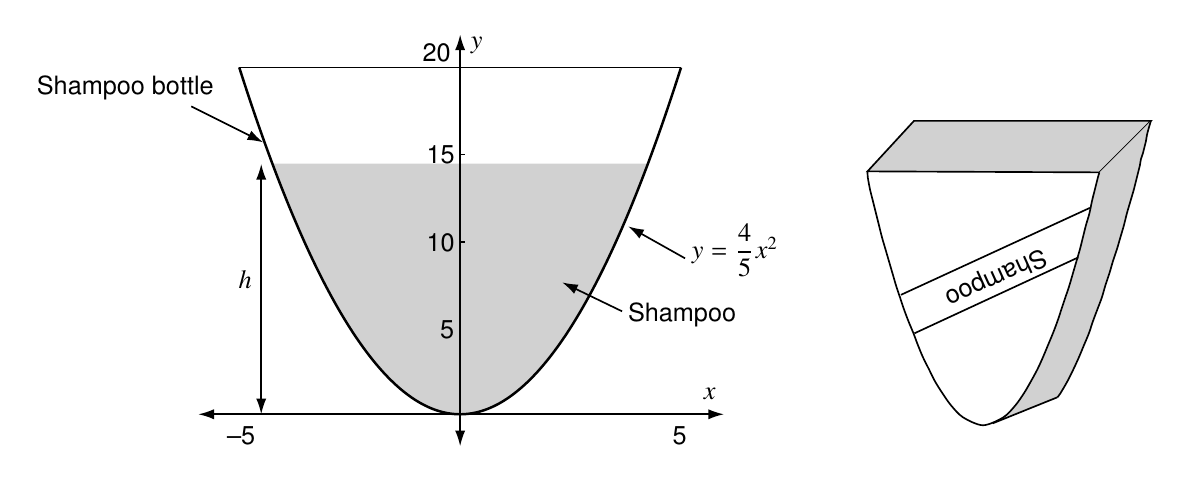
\begin{tikzpicture}[x=0.0127cm, y=-0.0127cm, font=\fontsize{9.5}{11}\selectfont, sl/.style={font=\fontsize{9.6}{11}\sffamily}]
  % 2D cross-section: vertex (439,407), 44.2 px per x unit, 17.35 px per y unit
  \def\ox{439}\def\oy{407}\def\sx{44.2}\def\sy{17.35}
  \fill[shade] plot[smooth, samples=60, domain=-4.25:4.25, variable=\u] ({\ox+\sx*\u},{\oy-\sy*0.8*\u*\u}) -- cycle;
  \draw[<->] (177,407) -- (703,407);
  \draw[<->] (439,439) -- (439,27);
  \foreach \r in {147,234.5} \draw (439,\r) -- (444,\r);
  \draw[line width=0.9pt, smooth, samples=90, domain=-5:5, variable=\u] plot ({\ox+\sx*\u},{\oy-\sy*0.8*\u*\u});
  \draw (218,60) -- (660,60);
  \draw[<->] (240,156.5) -- (240,407);
  \node[sl] at (415.5,46) {20};
  \node[sl] at (419.5,148) {15};
  \node[sl] at (419.5,235.5) {10};
  \node[sl] at (426,323) {5};
  \node[sl] at (220,428.5) {--5};
  \node[sl] at (658.5,428.5) {5};
  \node at (688,387) {$x$};
  \node at (455.5,38) {$y$};
  \node at (224,272.5) {$h$};
  \node[sl] at (104,80.5) {Shampoo bottle};
  \draw[->] (170,99) -- (242,135);
  \node at (714,243) {$y=\dfrac{4}{5}x^2$};
  \draw[->] (664,251) -- (607,219);
  \node[sl] at (661,307.5) {Shampoo};
  \draw[->] (601,304) -- (541,275);
  % 3D inverted bottle
  \filldraw[shade] (846.5,164) -- (893,113.5) -- (1130,113.5) -- (1078.5,165) -- cycle;
  \fill[shade] plot[smooth] coordinates {(1078.5,165) (1077,170) (1074,182) (1071,194) (1068.5,206) (1065,218) (1062,230) (1059,242) (1055.5,254) (1052,266) (1048.5,278) (1044.5,290) (1040.5,302) (1036.5,314) (1032,326) (1027,338) (1022,350) (1016.5,362) (1010,374) (1003,386) (994.5,398) (982.5,410) (970,416.5)}
     -- (1036.5,390) -- plot[smooth] coordinates {(1039.5,386) (1046.5,374) (1052.5,362) (1058,350) (1063,338) (1068,326) (1072,314) (1076.5,302) (1081,290) (1084.5,278) (1088.5,266) (1092,254) (1096,242) (1099.5,230) (1103,218) (1106,206) (1109.5,194) (1113,182) (1116,170) (1117.5,164) (1119,158) (1120,152) (1122,146) (1123.5,140) (1125,134) (1126,128) (1127.5,122) (1130,113.5)} -- cycle;
  \draw plot[smooth] coordinates {(846.5,164) (846.8,170) (849,182) (852,194) (855,206) (858,218) (861,230) (864.5,242) (868,254) (871.5,266) (875,278) (879,290) (883,302) (887.5,314) (892.5,326) (897,338) (902,350) (908,362) (914,374) (921.5,386) (930,398) (942,410) (962,418) (982.5,410) (994.5,398) (1003,386) (1010,374) (1016.5,362) (1022,350) (1027,338) (1032,326) (1036.5,314) (1040.5,302) (1044.5,290) (1048.5,278) (1052,266) (1055.5,254) (1059,242) (1062,230) (1065,218) (1068.5,206) (1071,194) (1074,182) (1077,170) (1078.5,165)};
  \draw plot[smooth] coordinates {(1036.5,390) (1039.5,386) (1046.5,374) (1052.5,362) (1058,350) (1063,338) (1068,326) (1072,314) (1076.5,302) (1081,290) (1084.5,278) (1088.5,266) (1092,254) (1096,242) (1099.5,230) (1103,218) (1106,206) (1109.5,194) (1113,182) (1116,170) (1117.5,164) (1119,158) (1120,152) (1122,146) (1123.5,140) (1125,134) (1126,128) (1127.5,122) (1130,113.5)};
  \draw (1036.5,390) -- (972,416);
  \draw (880,287.5) -- (1069,200.5);
  \draw (893.5,326) -- (1057.5,250);
  \node[sl, rotate=204.4] at (974.5,269.5) {Shampoo};
\end{tikzpicture}
\end{document}
